\chapter{Develop your own analysis}\label{chap:DevelopNewAnalyses}

This chapter explains step-by-step how to develop and run your own Harmony analyses.



%\section{Run Harmony}\label{sec:RunInEclipse}
%
%	\begin{itemize}
%		\item Go to \texttt{File $\rightarrow$ Import}
%		\item Select \texttt{Launch Configurations} under the \texttt{Run/Debug} category and click on \texttt{Next}
%		\item Click on \texttt{Browse} to select the \emph{configuration} directory located in the \emph{HarmonyWorkingDirectory}
%		\item Select the file \emph{Harmony.launch} as shown in figure \ref{} and click on \texttt{Finish}
%		
%	\end{itemize}
%
%Eclipse uses \emph{Run configurations} in order to know what should be launched and how : which plugins, which execution environment,... A default \emph{Run configuration} is provided in the \texttt{harmony.core} plug-in. In order to use it you have to import the \texttt{harmony.core} plug-in from your Eclipse installation into your workspace. 
%
%You can do this via the \texttt{File $\rightarrow$ Import} menu. Then select \texttt{Plug-ins and Fragments} (see figure \ref{fig:coreBundleImportMenu}). 
%
%In the \texttt{Import Plug-ins and Fragments} wizard, select \texttt{Import As $\rightarrow$ Project with source folders} as shown in figure \ref{fig:coreBundleImportMenu}.
%
%	\begin{figure}[H]
%		\centering
%		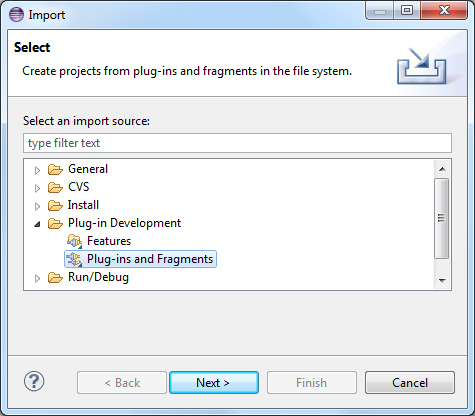
\includegraphics[width=.49\linewidth]{import-menu}
%		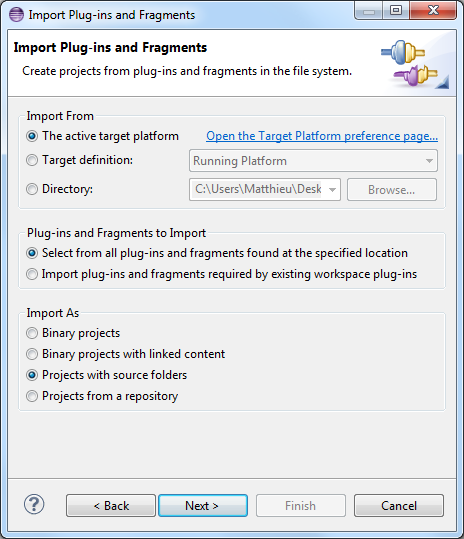
\includegraphics[width=.49\linewidth]{import-plugin-menu}
%		\caption{Menu for the importation of plugins in the workspace}
%		\label{fig:coreBundleImportMenu}
%	\end{figure}
%
%In the next step, add the \emph{fr.labri.harmony.core} plug-in in the list of \emph{Plug-ins and Fragments to Import}. You may use the filter box with "fr.labri" in order to find more rapidly the \emph{fr.labri.harmony.core} plug-in as demonstrated in figure \ref{fig:coreBundleImportSelection}.
%
%	\begin{figure}[H]
%		\centering
%		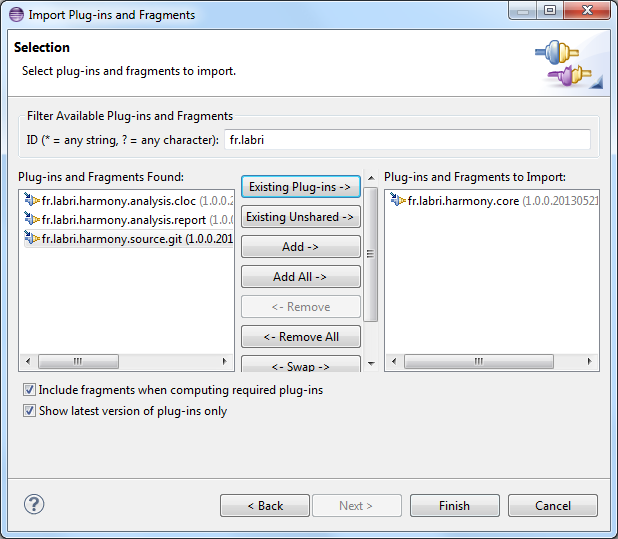
\includegraphics[width=.8\linewidth]{import-plugin-selection}
%		\caption{Selection of the Harmony core plugin for importation}
%		\label{fig:coreBundleImportSelection}
%	\end{figure}
%
%Finally press \texttt{Finish}. A new project has been added to your workspace. You may have build errors, in such a case you need to clean the project via the \texttt{Project $\rightarrow$ Clean} menu.
%
%We will be able to run Harmony in a few steps. The next thing to do is to copy the \texttt{configuration} directory --located in the \texttt{resources} directory from the \texttt{fr.labri.harmony.core} plugin-- into the root of workspace, where you should have a \texttt{.metadata} directory and the plug-in you imported:\\
%
%\begin{lstlisting}[language=bash]
%drwx------+ 1 XXXXXX None 0 21 mai   11:27 .metadata/
%drwx------+ 1 XXXXXX None 0 21 mai   14:09 configuration/
%drwx------+ 1 XXXXXX None 0 21 mai   13:08 fr.labri.harmony.core/
%\end{lstlisting}
%
%
%Then go back into Eclipse, and open the \texttt{Run Configurations} window (via the \texttt{Run} menu). In the left menu, you should see an \texttt{HarmonyEquinox} configuration under the \texttt{OSGi Framework} node as shown in figure \ref{fig:run-configurations}. Select it.
%
%You can now see a list of plugins. The ones that are selected are the ones that will be loaded if you launch this \emph{Run configuration}. Now, uncheck the "Show only Selected" checkbox (on the right) and type "fr.labri" in the filter box located at the top of the plugins list. Add the harmony plugins that are not imported in your workspace (i.e. reporting, cloc, and source.git) as shown in figure \ref{fig:run-configurations}. Remember that if you develop new analyses, you must update your \emph{Run configuration} by adding the new plugin otherwise you will not be able to run your analysis.
%
%	\begin{figure}[H]
%		\centering
%		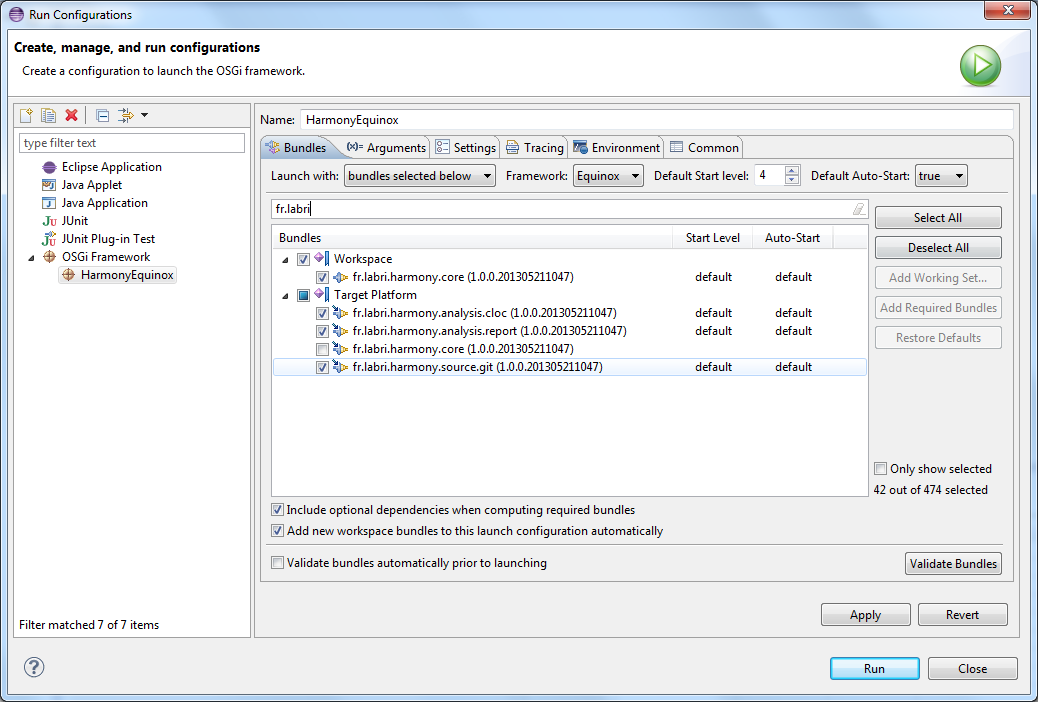
\includegraphics[width=.85\linewidth]{run-configurations}
%		\caption{Set up of the run configuration}
%		\label{fig:run-configurations}
%	\end{figure}
%
%Finally you can hit \texttt{Run} to launch the selected plugins. Once the OSGi console is loaded, type \texttt{harmony} (see figure \ref{fig:run-harmony}.
%
%	\begin{figure}[H]
%		\centering
%		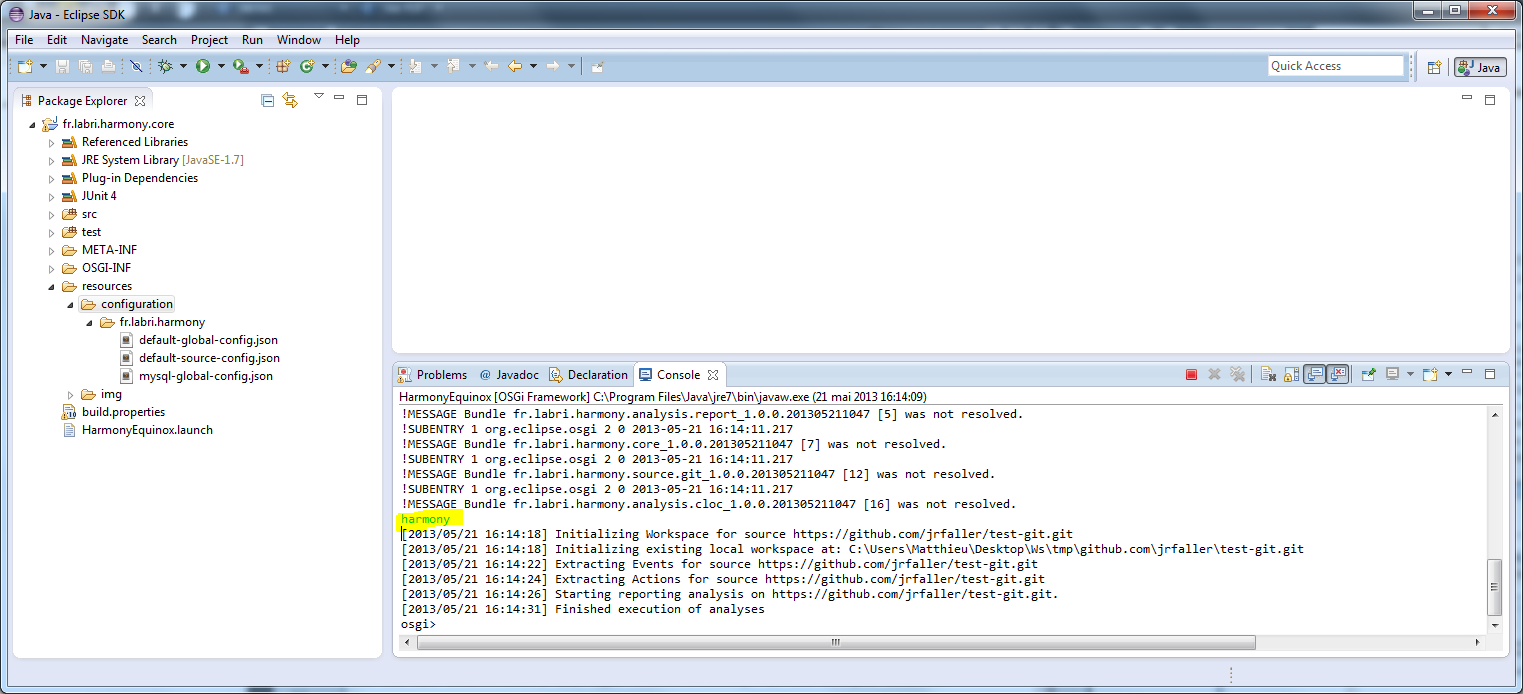
\includegraphics[width=.95\linewidth]{run-harmony}
%		\caption{OSGi console with Harmony running}
%		\label{fig:run-harmony}
%	\end{figure}


\section{Create a new analysis}

Now that your development environment is ready and that you know how to run analysis within Eclipse. We will see how you can create your own analysis. There are two ways of doing so, the easy way by using the dedicated wizard (see section \ref{newAnalysis:wizard}) and the hard way by creating the project from scratch (see section \ref{newAnalysis:fromScratch}). In both cases do not forget to add your new analysis to your \emph{Run Configuration} (see previous section).

\subsection{Using the wizard}\label{newAnalysis:wizard}

Make a right-click on the \emph{Project Explorer} view and select \texttt{New $\rightarrow$ Project}. As shown in figure \ref{fig:wizard-selection} select the \emph{analysis} wizard located in the \emph{Harmony} category and click on \emph{Next}.

Now you should see something a form similar to the figure \ref{fig:wizard-new-analysis-form} that ask you details about the analysis you want to create. The \emph{project name} must follow the Java package naming convention as the project name will be used as your root package as well as your plugin unique identifier. The \emph{Analysis class name} is the name of the class that will implement the analysis service trough the method \emph{runOn(Source src)}. Press \emph{Finish}.

Implement you analysis in the method \emph{runOn(Source src)}. Take a look at existing analyses for inspiration. Follow the same procedure as the one you have followed for importing the \emph{fr.labri.harmony.core} (see section \ref{sec:RunInEclipse}). Finally you can run it by modifying your configuration files (see Chapter \ref{chap:AdvancedUse}) and your \emph{Run Configuration} (see Section \ref{sec:RunInEclipse}).


	\begin{figure}[H]
		\centering
		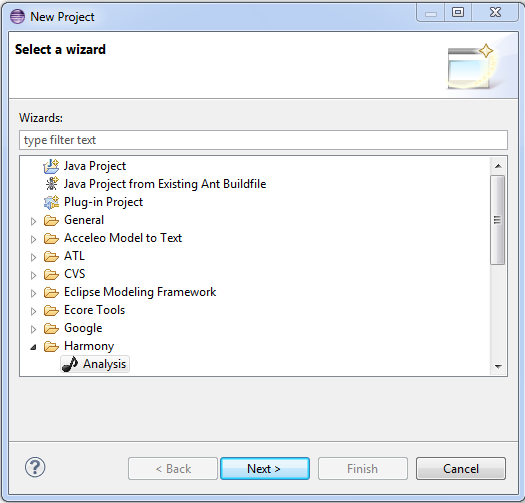
\includegraphics[width=.7\linewidth]{wizard-selection}
		\caption{Selection of the Harmony wizard for creating a new analysis}
		\label{fig:wizard-selection}
	\end{figure}
	
	\begin{figure}[H]
		\centering
		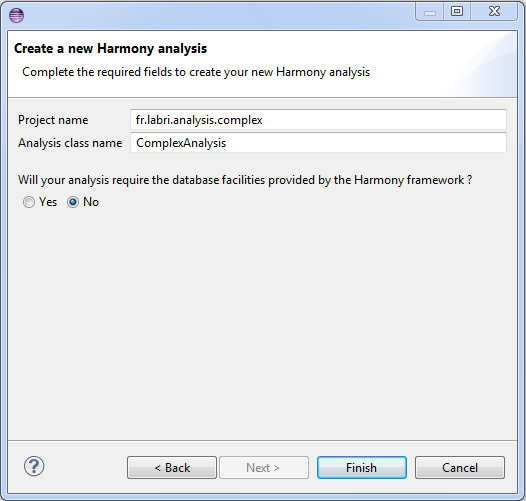
\includegraphics[width=.7\linewidth]{wizard-new-analysis-form}
		\caption{Form of the wizard for creating a new analysis}
		\label{fig:wizard-new-analysis-form}
	\end{figure}


\subsection{Starting from scratch}\label{newAnalysis:fromScratch}

If for some inexplicable reason you want to create your analysis project from scratch, this section will guide you. The first step is to create a plug-in project for this analysis. Make a right-click on the \emph{Project Explorer} view and select \texttt{New $\rightarrow$ Project $\rightarrow$ Plug-in Project} and \emph{Next}. You a wizard similar to the one presented in figure \ref{fig:new-plug-in}. For demonstration purpose we will call it \texttt{dummy}. Set the target platform to use the Equinox OSGi framework and press \emph{Next}.

	\begin{figure}[H]
		\centering
		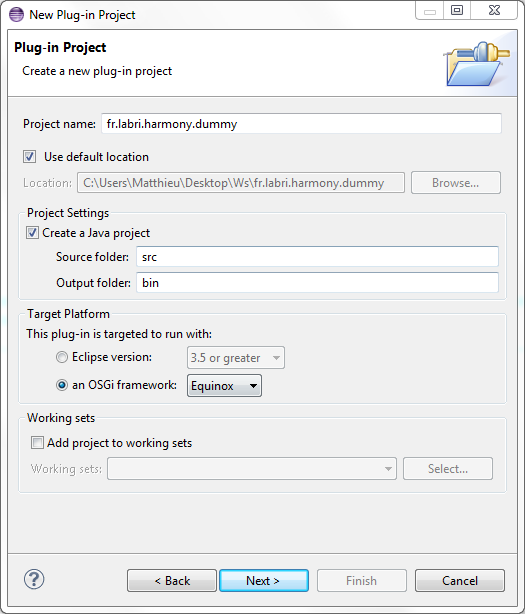
\includegraphics[width=.7\linewidth]{new-plug-in}
		\caption{First page of the plug-in wizard}
		\label{fig:new-plug-in}
	\end{figure}
	
Press next. You should now see the \texttt{Content} form as shown in figure \ref{fig:plug-in-content}, uncheck the \texttt{Generate an activator...} checkbox. Finally press \emph{Finish} to create your new project.

	\begin{figure}[H]
		\centering
		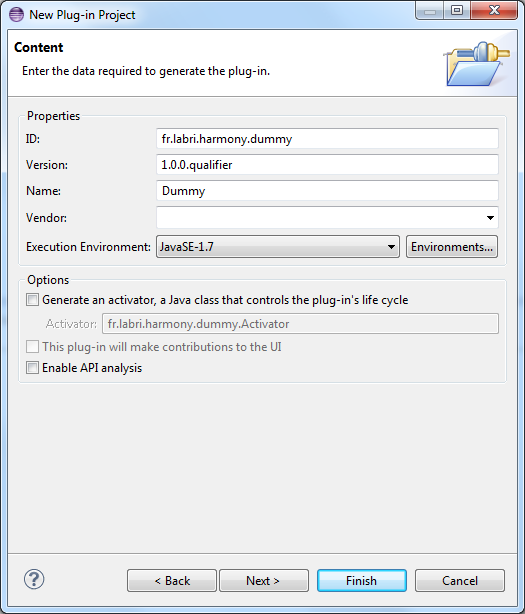
\includegraphics[width=.7\linewidth]{plug-in-content}
		\caption{First page of the plug-in wizard}
		\label{fig:plug-in-content}
	\end{figure}

In order for your analysis to use the harmony framework, you need to add the corresponding dependencies to your plug-in configuration. If it is not already the case open the \texttt{MANIFEST.MF} file located in the \texttt{META-INF} folder. Open the \texttt{Dependencies} tab, and add the following imported packages:

\begin{lstlisting}
fr.labri.harmony.core
fr.labri.harmony.core.analysis
fr.labri.harmony.core.config.model
fr.labri.harmony.core.dao
fr.labri.harmony.core.log
fr.labri.harmony.core.model
javax.persistence
\end{lstlisting}

You should obtain a configuration similar to the one presented in figure \ref{fig:harmony-dependencies}

	\begin{figure}[H]
		\centering
		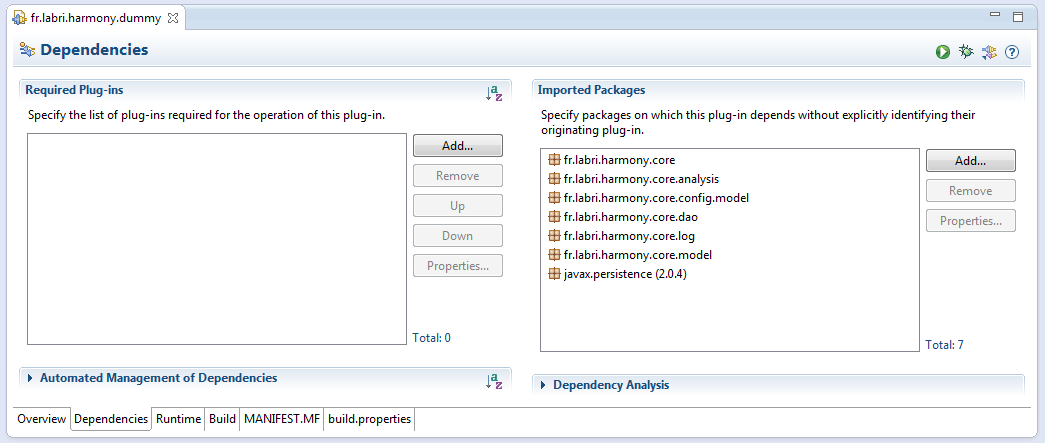
\includegraphics[width=\linewidth]{harmony-dependencies}
		\caption{First page of the plug-in wizard}
		\label{fig:harmony-dependencies}
	\end{figure}

You now have to add your analysis main class that will implement the \emph{AbstractAnalysis} class defined in the Harmony Core. To do so, use the Eclipse \emph{new class} wizard, and check the \texttt{Constructors from superclass} checkbox as shown in the figure \ref{fig:new-java-class}. 

	\begin{figure}[H]
		\centering
		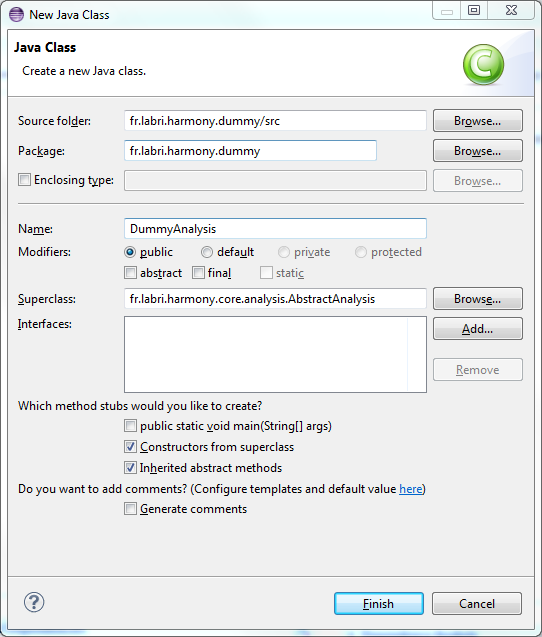
\includegraphics[width=.7\linewidth]{new-java-class}
		\caption{Creation of the main class of class of your analysis}
		\label{fig:new-java-class}
	\end{figure}

This is very important, as \textbf{both constructors from AbstractAnalysis are mandatory}. Also add as your superclass: \\ \emph{fr.labri.harmony.core.analysis.AbstractAnalysis}\\
Press \emph{Finish}. You should have something looking like the class presented in the listing \ref{code:dummyAnalysis}. The method \emph{runOn(Source src)} is where you must implement your analysis. Take a look at existing analyses for inspiration. Follow the same procedure as the one you have followed for importing the \emph{fr.labri.harmony.core} (see section \ref{sec:RunInEclipse}).

\includeSourceFile{resources/listings/DummyAnalysis.java}{DummyAnalysis lass}{code:dummyAnalysis}{java}

You now have a class that implements the analysis service so you need to inform the OSGi runtime about your implementation. Create an empty folder called \emph{OSGI-INF} at the root of your project. Then create a new component definition : make a right-click on your plug-in project and select \texttt{New $\rightarrow$ Component Definition}. Complete the form by taking example of the figure \ref{fig:new-component}, for example the component definition should be in the newly created  \emph{OSGI-INF} folder. Finally press \emph{Finish}.

	\begin{figure}[H]
		\centering
		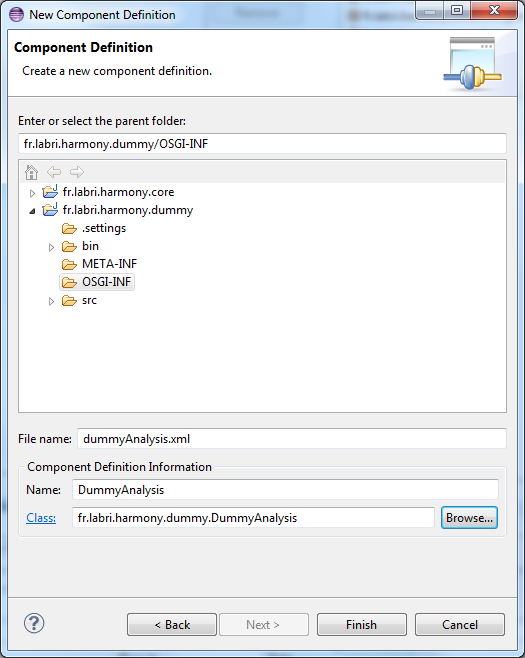
\includegraphics[width=.7\linewidth]{new-component}
		\caption{Wizard for creating a new component definition}
		\label{fig:new-component}
	\end{figure}
	
Open the newly created file and go the \emph{Service} tab as shown in the figure \ref{fig:provided-services}. Click on the \emph{Add} button of the \emph{Provided Services} section and select \texttt{fr.labri.harmony.core.analysis.Analysis}, press \emph{Ok}.
	
	\begin{figure}[H]
		\centering
		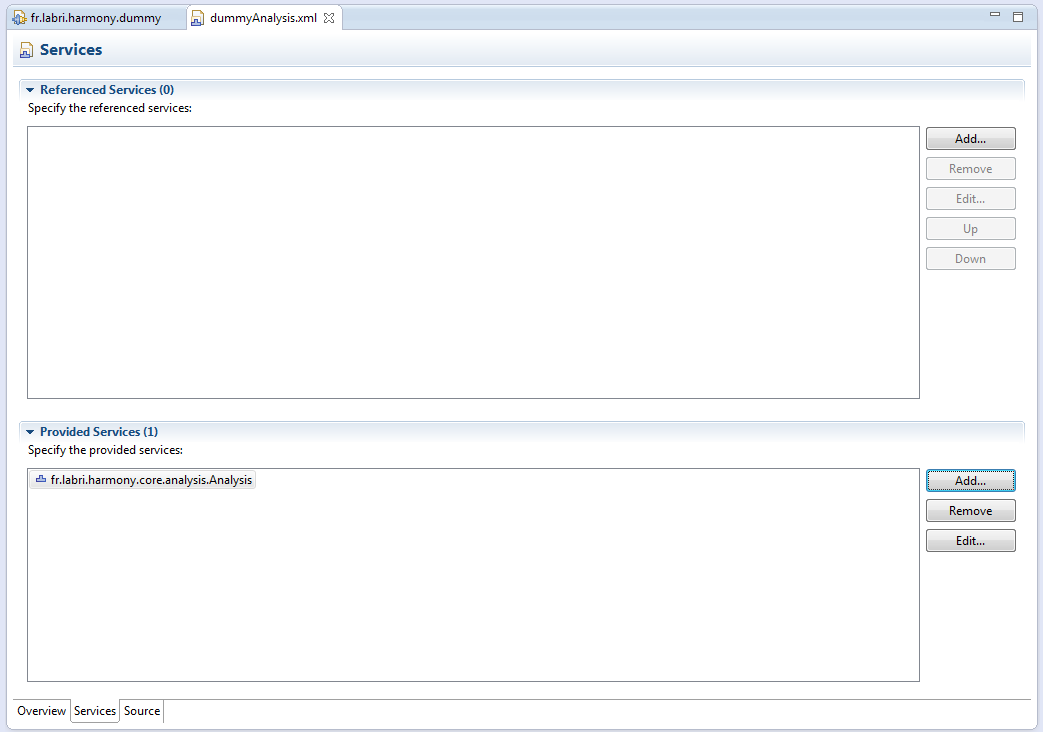
\includegraphics[width=\linewidth]{provided-services}
		\caption{Provided services}
		\label{fig:provided-services}
	\end{figure}
	
Your analysis project is now set up. You can run it by modifying your configuration files (see Chapter \ref{chap:AdvancedUse}) and your \emph{Run Configuration} (see Section \ref{sec:RunInEclipse}).

%
%\section{How to write an analysis}
%
%	\subsection{The Harmony model}
%	
%		\begin{figure}[H]
%			\centering
%			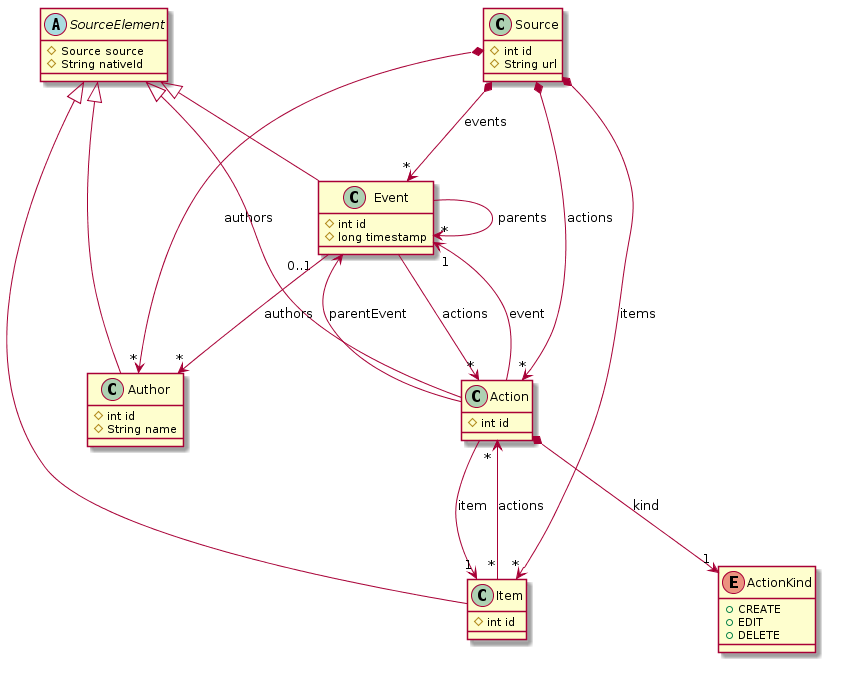
\includegraphics[width=\linewidth]{data-model}
%			\caption{Class diagram of the main concepts of the Harmony generic data model}
%			\label{fig:data-model}
%		\end{figure}
%	
%	\subsection{Using the database}
%	
%	\subsection{Output management}
	
% TODO explain the use of the dao
%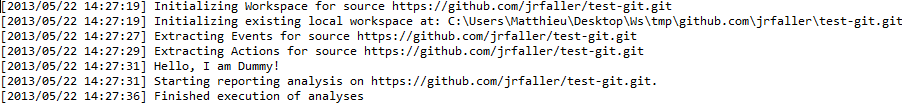
\includegraphics[width=6in]{dummy-execution}
%
%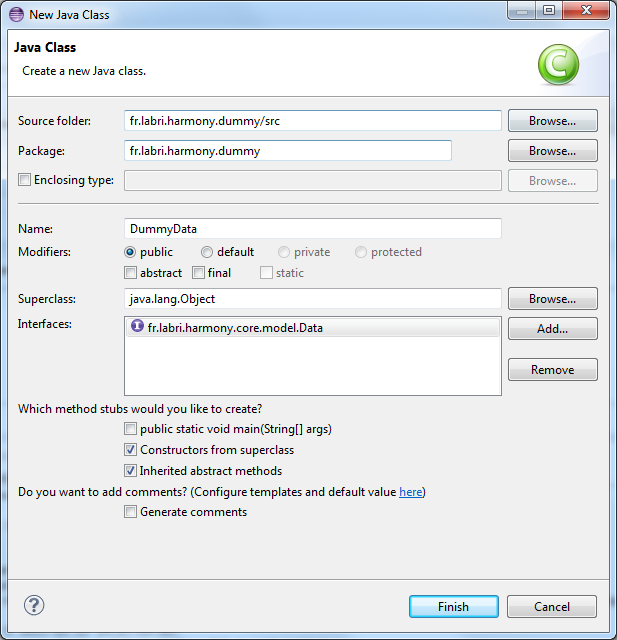
\includegraphics[width=6in]{new-data-class}
%
%
%\begin{lstlisting}[language=Java]
%DummyData d = new DummyData();
%d.setContent("plop");
%dao.saveData(this, d, Data.SOURCE, src.getId());
%\end{lstlisting}




